\subsection{Aplicação Fábrica: Executar Analise}
\subsubsection*{Descrição do caso de uso}
Uma analise é um script SQL com uma query personalizada. Para executar uma analise basta pressionar o botão executar na linha referente à analise pretendida.

\subsubsection*{Models compatíveis com o caso de uso}
Este caso de uso é apenas compatível com o model Analises.

\subsubsection*{Fluxo do caso de uso}
O caso de uso inicia-se quando o utilizador pressionar o botão executar da linha do registo que pretende executar. A página vai recarregar, fazendo aparacer o resultado da analise pedida.


\begin{figure}[H] 
	\begin{center}
		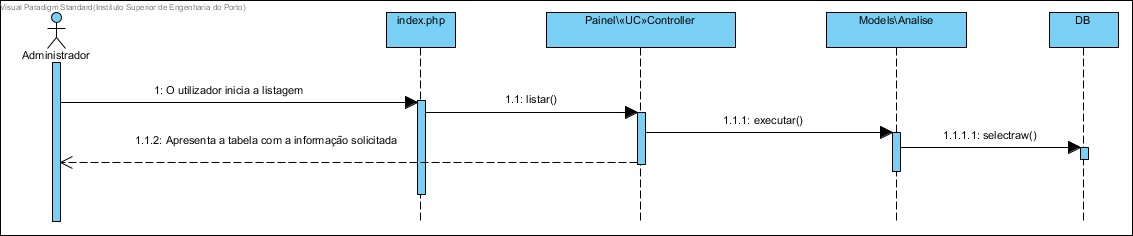
\includegraphics[width=\textwidth,keepaspectratio]{figuras/Diagramas_vp/SD_Painel_7_Executar_Analise.jpg}
		\caption{Diagrama de sequência para executar uma recolha}
		\label{fig:sd_executar analise} 
	\end{center}
\end{figure}